\documentclass[11pt]{article}
\usepackage[top=1.00in, bottom=1.0in, left=1.1in, right=1.1in]{geometry}
\usepackage{Sweave}
\renewcommand{\baselinestretch}{1.1}
\usepackage{graphicx}
\usepackage{natbib}
\usepackage{amsmath}
\usepackage{gensymb}
\usepackage{parskip}
\usepackage{xcolor}
\usepackage{xr-hyper}
\usepackage[utf8]{inputenc}
\externaldocument{grephonms}
\usepackage{longtable}

\def\labelitemi{--}
\parindent=0pt

\begin{document}

\renewcommand{\refname}{\CHead{}}

% See also: git/grants/crc2023/crc2023app/docs/crc_notes2023more.tex which has some reference notes

\title{Supplement: Why longer seasons with climate change may\\ not increase tree growth}
% \author{Team Grephon}
\date{\today}
\maketitle

\renewcommand{\thetable}{S\arabic{table}}
\renewcommand{\thefigure}{S\arabic{figure}}


\section*{Literature review methods}

We conducted a review to find papers focused on relationships between growing season length and tree wood growth, though contrasting terminology made it challenging to identify papers through one search. After reviewing several recent papers \citep{dow2022warm,zohner2023effect}, we searched ISI Web of Science for ``growing season length" AND ``tree ring*" (ALL FIELDS) on 12 April 2023, which returned 33 citations. We next reviewed abstracts from these papers and discarded ones that did not mention the relationship between growing season length and growth. We further reviewed all citations within all papers for additionally relevant papers and included them in our review following the same criteria of reviewing abstracts and including papers that mentioned they tested or examined the relationship between growing season length and tree growth. Papers needed at least one metric related to growing season length and one metric related to growth to be included (and these could not be the same metric) but we did not require they clearly measure season length (end and start) to be included. In total we report on 36 papers after reviewing over 107 potentially relevant papers and discarding one paper from which we scraped data but found it did not meet our criteria \citep[][because it used tree rings as a metric of both growth and growing season length]{bruening2017}. % These ISI methods in outline.tex % grephon_warmingexpts also has some ISI searches, but no date and is focused on warming experiments. 107 is the number in the articles folder. 
% on 31 Oct 2023, I tried ISI (Web of Science Core Collection) for SEARCH tree OR woody (All Fields) and growth (All Fields) and growing season length (All Fields), which returned 886 references. 
% Average number of papers in ecological meta-analysis: 24 papers see https://esajournals.onlinelibrary.wiley.com/doi/abs/10.1002/ecy.3680

Once a paper was included, we aimed to record all studies from it related to season length and growth (e.g. a paper might include a global study of satellite metrics of start of season and productivity as well as an experiment; these would be considered two separate studies within one paper). Given the large diversity of metrics we found, we did not extract quantitative estimates of growing season length, growth, or their relationship. Instead, we extracted data on location, species, how they measured growing season length, growth, what relationship they found and what internal and external drivers they mentioned (full dataset with metadata details for each column available on the Knowledge Network for Biocomplexity at publication). 

Papers often reported dozens or more statistical tests from different analyses of data or different types or subsets of data, thus we recorded a unique observation (that is, one recorded row of data for our literature review) within each study when papers reported: (1) distinctly different datasets (e.g., a global analyses of observations and a short-term experiment); (2) multiple distinctly different measures of growth (e.g., tree ring width and flux tower) and/or growing season length (e.g., they reported both end of season as budset and end of wood growth through xylogenesis); (3) distinctly different results for growth $\times$  growing season length depending on metric (e.g., using budset for growing season length they find a growth $\times$ growing season length relationship, but using leaf coloring they do not). % Numerous studies in the review reported multiple metrics of growth and for end of season (e.g., budset versus leaf coloring) and found differing relationships between growth and growing season length depending on the  definition; in these cases we reported all combinations per study. 

% Methods below adapted from https://github.com/lizzieinvancouver/grephon/issues/29
We returned to the papers to also assess them for which hypotheses they addressed. For this, we reviewed papers for stated hypotheses and/or analogous research questions that were specifically addressed in the results (e.g. hypothesis testing).  After this we grouped each hypothesis to a broader main hypothesis (or hypothesis cluster) displayed in Fig. 1, save for hypotheses including $CO_2$ limitation, which is not shown but mentioned in three papers (see Table \ref{tab:ref}). We extracted all hypotheses/questions from each paper, resulting in many papers addressing multiple hypotheses (11 of 36 papers). 

\subsection*{Trends with year}
% See whathappened.R and look for # Trends across years analysis
Across studies which found support for or against a relationship between growth and growing season length (40 of 59 total studies) the range of years was very similar: spanning 2000 to 2023 with a mean of 2017 for studies that found a positive relationship and spanning 2012 to 2023 with a mean of 2020 for studies that did not. Further, we found no trend through time for finding a positive or negative relationship  (estimated slope from logistic regression overlapped 0). 

\section*{Growth $\times$ elevation relationships}

Using Google Scholar and ISI Web of Science, we searched the literature for studies of tree growth, especially via diameter or ring width, by elevation or latitude. Of 20 papers we found for these relationships, six included clear raw tree data in either scatterplots or tables that we scraped: \citet{oleksyn1998growth,huang2010radial,cavin2017highest,wang2017climatic,zhu2018spatial,zhou2022altitudinal}. 

We could not scrape data from 14 papers for the following reasons: 
\begin{enumerate}
\item Absence of observational tree growth raw data: Some studies only presented the correlation or the data was modeled. 
\item  Measures other variables: Some studies examined leaf area index and forest NPP. 
\item  Standardization of tree growth with other variables: Papers did not present the raw data (e.g., papers presented the data calculated with other variables).
\item  Presence of overlapping data points: Data points in the plots presented were not visually identifiable for accurate data scraping.
\item Line graphs: No discrete data points for image processing. 
\item Geographical scale: The locations of data collection spread across large longitudinal or latitudinal gradient. 
\end{enumerate}

We scraped tree growth data from the selected studies using the Fiji image processing package with the Figure Calibration plugin. We calibrated $x$ and $y$ axes using the Figure Calibration plugin, followed by measuring growth values at different elevation using the measure function in Fiji. Of the six remaining papers, we show results for three, excluding \citet{huang2010radial} because it included only results for trends by latitude (and most other studies included only trends by elevation), and \citet{cavin2017highest,zhu2018spatial} because the elevation co-varied with latitude. % So the three we show are: \citep{oleksyn1998growth,wang2017climatic,zhou2022altitudinal}

Thus, we show data from: \citet{oleksyn1998growth}, which measured 54 populations of  \emph{Picea abies} along 8 altitudinal transects in Southern Poland, we present the mean DBH (cm yr$^{-1}$) of values collected from each population (although 54 populations were monitored, only 42 data points were clearly visible in Figure 2 in the paper); \citet{wang2017climatic}, which collected  tree cores (37-100 years) collected from 4 different sites across an elevation gradient in the Luyashan Mountains in North China, we present the median of tree ring width values from the collected cores (147 tree cores collected from 73 trees); and \citet{zhou2022altitudinal}, who collected tree ring width data (cores of 60-80 years) of \emph{Pinus yunnar} from 6 altitudinal transects in Yunnan, China; we present the median of tree ring width of each transect.

\section*{The challenge of metrics: Measuring growth and growing season length}

Understanding the diverse drivers and testing underlying hypotheses (Fig. 1) for growth $\times$ season length relationships requires a common language. We found 14 different metrics of start of season, 16 metrics of end of season (25 metrics of growing season length), and 21 different metrics of growth across 59 studies---highlighting just part of the problem (see also \emph{Box: Growth, season length and the challenge of standardized metrics} in the main text). Definitions and metrics for external and internal drivers were myriad, %CJC 15Dec - I think we could again add numbers for external and internal divers, clarifying these were after systematically assigning studies into groups
with papers reporting dozens of tests of different aspects of climate over different temporal windows. Although this is understandable given the differing goals of these papers, it also slows progress. 

A common framework for explanatory and response variables would accelerate research by easing communication between fields and providing a path to comparable quantitative estimates. 
This should also include expected statistical tests, as we found a number of papers failed to directly test for growth $\times$ growing season length relationships (Fig. 2), often instead testing only certain hypothesized indirect relationships \citep[e.g. spring temperature $\times$ growth in][]{dow2022warm}. % A first fundamental need for any framework is comparable quantitative estimates---which we currently lack. 

\subsection*{Measuring growth}

Tree growth can be defined and measured in a variety of ways. It is often divided into primary (growth from the root and shoot tips that results in increased height and length) versus secondary (growth that increases the thickness or girth of stems and branches above ground, as well as below ground parts), or leaf production versus wood production. Across studies, we found the largest proportion used metrics related to secondary growth ($n=$28), followed by primary growth ($n=$20), with a smaller number using metrics that reflected combined primary and secondary growth ($n=$9), and root:shoot ratio ($n=$1, see also \emph{Box: Growth, growing season length and the challenge of standardized metrics} in the main text).  Some studies used modeled estimates of photosynthesis (e.g., \citet{smith2014implications} relied on daily photosynthesis estimates derived from the LPJ-GUESS photosynthesis model, while \citet{chen2000approaches} estimated photosynthesis using the Integrated Terrestrial Ecosystem C-budget model, InTEC). 
Others measured photosynthesis at the leaf level, through flux towers, or used greenness metrics (NDVI). 

Growth measurements varied across disciplines and study types, posing further challenges to an interdisciplinary approach to understanding how growing season length relates to growth. 
Greenhouse or growth chamber studies and provenance trials were more likely to measure height or biomass, whereas larger scale syntheses and remote-sensed studies are more likely to use metrics of carbon assimilation. 
The inconsistency of current metrics across fields is not surprising, but may be confusing---including photosynthesis as a metric of growth may seem unconventional for ecophysiologists, for example, who may interpret the process of photosynthesis as distinct from growth---and also stalls progress toward a unified model across disciplines.

Aligning across the range and scale of growth metrics will be critical for an integrated understanding of growth-growing season length relationships and implications under continued climate change.  
There is decoupling among some metrics of growth, as different types of growth (leaves, shoots, wood) have different phenologies within a season, and may vary across years, as well (e.g., with different lags, Fig. \ref{fig:gxelev}).
For example, vegetation photosynthesis may be poorly correlated with tree radial growth, and this relationship can vary seasonally \citep{cabon2022cross}. 
Further, tree radial growth is not a perfect indicator of whole tree growth, since plants allocate carbon to their roots, leaves, reproductive structures, and stores in addition to aboveground biomass. 
Relationships among different metrics of growth are not simple, so selecting relevant ones and aligning across the most widely used ones will be necessary, though not easy: the relationship  between photosynthesis, radial growth, and carbon uptake has large implications for future carbon sequestration and it remains widely debated \citep{green2022limits}. 
Further, there is a need to understand how to scale up across these varying metrics- from leaf and individual level to populations, communities, and ecosystems- while incorporating the variation that exists within and across levels.

\subsection*{Measuring growing season length}

Growing season length is defined in myriad ways due to varying definitions and metrics for the start of season and the end of season. For example, the end of season could be defined as budset, representing the end of vegetative phenology, or as xylogenesis, representing the end of wood phenology. Additionally, in our literature review, we found several studies that leveraged climate data as a proxy for start or end of season metrics, such as snowmelt for start of season or growing season GDDs. We therefore grouped all reported growing season length metrics into four separate categories: 1) `Climate and date' simulated by climate data, 2) `Vegetative phenology' through field observations or satellite derived measurements, 3) `Wood phenology' measured by dendrometers and xylogenesis, and 4) not measured, which includes all studies that only measured start or end of seasons but not both. 

\section*{Extending disciplinary focus to help bridge the internal-external drivers divide} 

% Careful interdisciplinary is critical, but will benefit from shifts within disciplines. 
% Standardized measurements will not yield fully comparable estimates---especially on the relative impacts of external and internal drivers---without larger shifts within fields. We found that dendrochronology considers almost exclusively external climatic drivers, while physiological tests of internal constraints do not usually make predictions that scale up easily beyond the lab or greenhouse. Major fields studying this relationship---dendrochronology, phenology research and physiology---all need to broaden in specific ways to overlap with one another to facilitate interdisciplinary work. At the same time, all fields have missed certain major hypotheses they could test (Fig. \ref{fig:hypotheses}), highlighting the need to integrate perspectives from other disciplines with relevant theory and methods. 

Each field studying growth $\times$ growing season length today has its own historical aims, and thus, its own biases towards certain species, methods and metrics. For example, dendrochronology's original focus on using tree growth to estimate climate has led to sampling biases \citep[e.g. to `climate-sensitive' individual trees,][]{klesse2018sampling,nehrbass2014influence} and statistical detrending \citep{rollinson2021climate}, which may obscure patterns where the signal of longer growing seasons and biotic drivers may be most apparent (such as rapid growth phases). Dendrochronology also generally focuses on conifers \citep[gymnosperms,][]{zhao2019international}, creating a major split from most studies of leaf phenology, which focus almost entirely on deciduous angiosperm species (see Fig. \ref{fig:itrbdpep}). By contrast, phenology research has been strongly focused on spring events (e.g. budburst, leafout), with limited data on fall events and thus limited data to calculate growing season length. This focus on spring events may have been justified decades ago, when most shifts from anthropogenic warming occurred in the spring, but less justified as increasing research suggests important complexity in fall shifts \citep{gill2015,zohner2023effect} and a need to scale up phenological research to understand tree growth.

%[jhrl deleted this - was too long] led to certain assumptions and methods that may obscure the complexity of how growth shifts with growing season length. Fundamentally, the field relies on an assumed relationship that, within individual and populations of trees, growth (measured by annual ring width) is greater when growing conditions---climatically---are better \citep[e.g.][]{cook2013methods}.  Dendrochronologists' traditional aim to magnify this climate signal has led to standard approaches, including sampling biases \citep[e.g. to `climate-sensitive' individual trees,][]{klesse2018sampling,nehrbass2014influence} and statistical detrending \citep{rollinson2021climate}, that may obscure patterns where the signal of longer growing seasons and biotic drivers may be most apparent \citep[such as rapid growth phases,][]{manzanedo2019towards}.  %Fundamentally, the field has long assumed growth decreases with shorter growing seasons \citep[e.g.][]{bruening2017} over space, such as higher elevations and latitudes.%AKE: I have not read bruening but a skim of it suggests that it is not a tree ring paper- rather a treeline paper. do we still want to cite it here? I removed it but I can look for another one that is tree ring focused...
 % Bridging this gap would be aided by physiological studies reporting metrics similar to ring width, alongside their more common measurements of shoot elongation, height and biomass. 

These field-specific historical trends limit the opportunities for interdisciplinary insights. For example, dendrochronology studies generally eliminate much of the drivers that physiological studies focus on, while physiological studies often fail to make predictions that scale up (e.g., to adult trees or for diverse species). Opportunities to overlap dendrochronology time records with metrics of growing season length measured through vegetative phenology appear high (Fig. \ref{fig:itrbdpep}), but sampling biases towards conifers in one and angiosperms in the other field limit current opportunities. All fields could therefore benefit from tackling the challenge of understanding the physiological connections between growing season length and growth, and even the genetic and developmental underpinnings of these connections. To date, much work has focused on measures of growth and phenology without a clear mechanistic understanding of what triggers growth and its cessation, and how these triggers and responses have evolved.  %CJC 15 Dec - reference Fig S1 here - only 3 studies looked at external or internal factors by phenology.
Progress in this area could be particularly important for making projections, as extrapolating can be dangerous when the underlying mechanistic model is wrong. Physiological studies that follow carbohydrate balance and cell division \citep[see][]{locosselli2017dendrobiochemistry} versus growth dynamics could yield insights, as could additional work on xylogenesis---especially if done with a focus both to extrapolate to long-term tree ring studies and/or in physiological experiments \citep{fang2020physiological,simard2013intra}. Expanding beyond the current disciplines focused on this topic could also be informative. For example, a clearer physiological understanding of which environmental stimuli trigger leaf expansion, senescence, woody growth, and heartwood formation alongside an evolutionary perspective could advance understanding of growth
constraints \citep{baas2011wood,eckert2019makes,ensminger2015tree,juvany2013photo}.

% Biotic/spp diversity for all ... 
% All fields have lacked a focus on the ecology of growth $\times$ growing season length, generally ignoring impacts of certain external drivers, the complexity of life-history, and species differences. Dendrochronology often uses frost events or insect outbreaks as markers of particular years, but rarely integrates them into patterns of growth. A shift to reporting and estimating effects of frost events, biotic disturbances, and reproduction status of trees (including mast years) could provide new estimates of the effects of these drivers. Physiological studies tend to avoid such complexities through controlled environments and a focus on juvenile plant stages  \citep{poorter2016pampered}, but scaling up between life stages will be critical for useful models of growth, and to bridge to dendrochronology. % Both fields have also tended to ignore competition. Mechanistic physiology studies rarely measure or include competition and, given dendrochronology's focus on climatic signal through growth, the field similarly tries to avoid the study or impact of plant competition, even though it is foundational to forest dynamics.

% All fields would benefit from a deeper understanding of the physiological and/or developmental connections between growing season length and growth. Much work has focused on measures of growth and phenology without a clear mechanistic link. Similarly, many current suggestions of constraints lack any physiological mechanism. Physiological studies that follow carbohydrate and cell division versus expansion dynamics could yield insights. This is particularly important if want to include constraints in our projections, as extrapolating is especially dangerous when the underlying mechanistic model is wrong

\clearpage
\section*{Figures \& Tables}

% latex table generated in R 4.2.0 by xtable 1.8-4 package
% Sun Jan 26 16:21:27 2025
\begingroup\footnotesize
\begin{longtable}{p{0.3\textwidth}p{0.1\textwidth}p{0.40\textwidth}}
\caption{\textbf{Hypotheses and references for studies in our database.}} \\ 
  \hline
Hypothesis & Number of Studies & References \\ 
  \hline \endhead  \hline
longer season = more growth &  10 & \citep{camarero2022decoupled,chen2000,vcufar2015variations,delpierre2017tree,de2022temperature,gao2022earlier,grossiord2022warming,keenan2014net,silvestro2023longer,wheeler2016snow} \\ 
  warmer temperatures = more drought (drought limitation) &  10 & \citep{brand2022,buermann2018widespread,camarero2022decoupled,de2022temperature,drew2018growth,eckes2021,etzold2022number,kolavr2016response,oddi2022contrasting,zhu2021different} \\ 
  warmer temperatures = more growth &   8 & \citep{camarero2022decoupled,dow2022warm,finzi2020,moser2010timing,richardson2010influence,soolanayakanahally2013timing,stridbeck2022,zhang2021drought} \\ 
  shift of whole pheno sequence &   6 & \citep{delpierre2017tree,de2022temperature,richardson2010influence,soolanayakanahally2013timing,zani2020increased,zohner2020interactive} \\ 
  effect of growth rate not equal to growth duration &   5 & \citep{cuny2012life,de2022temperature,francon2020,michelot2012comparing,ren2019} \\ 
  internal constraints (including popl'n, photoperiod) &   5 & \citep{moser2010timing,sebazc2020,soolanayakanahally2013timing,vitasse2009altitudinal,zohner2023effect} \\ 
  carbon fertilization &   3 & \citep{chen1999effects,finzi2020,oddi2022contrasting} \\ 
  species-specific responses &   3 & \citep{cuny2012life,etzold2022number,michelot2012comparing} \\ 
  shift in allocation &   1 & \citep{mckown2016impacts} \\ 
  \hline
\label{tab:ref}
\end{longtable}
\endgroup
\begin{figure}[h!]
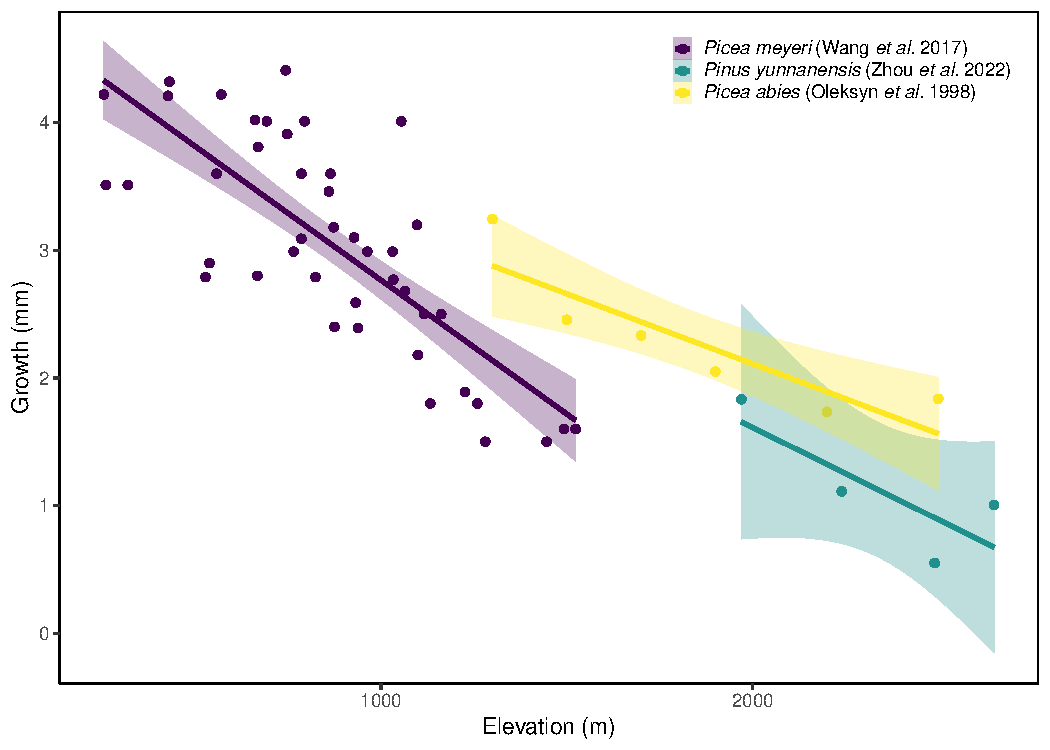
\includegraphics[width=0.7\textwidth]{..//analyses/growthxelevationetc/figures/growthbyelevation_plot.pdf} % {..//figures/_allfiguresFromRuben/growthbyelevation.png}   
\caption{Growth $\times$ elevation relationships from the literature with simple linear regression fits shown with 89\% confidence intervals. \citet{oleksyn1998growth} measured growth (mm) as diameter at breast height increments, while the other studies \citep{wang2017climatic,zhou2022altitudinal} measured growth (mm) as ring width. See `Growth $\times$ elevation relationships' section for more methods details.} % and Fig. \ref{fig:growelevMORA} for an example from one site.
\label{fig:gxelev}
\end{figure}

\begin{figure}[h!]
%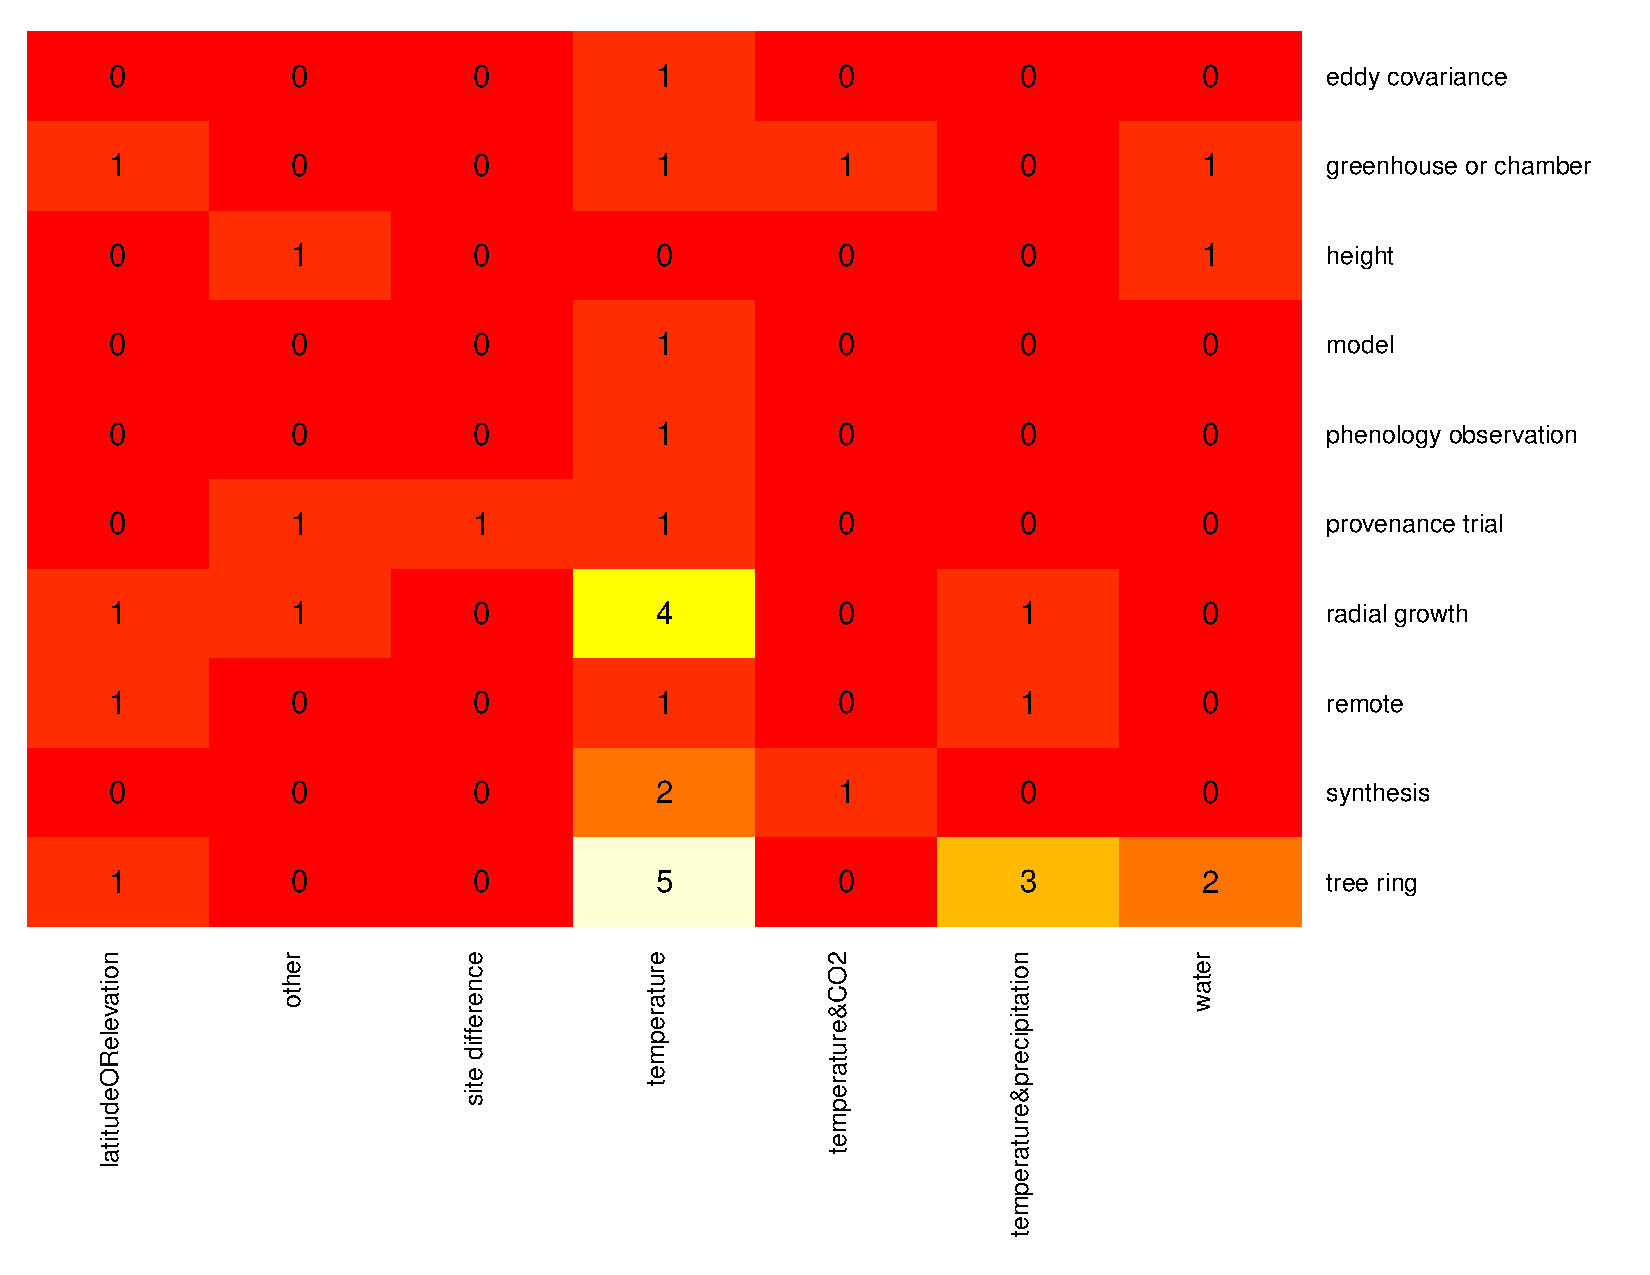
\includegraphics[width=0.8\textwidth]{..//figures/heatmaps/heatmap_extbymethod.pdf}
%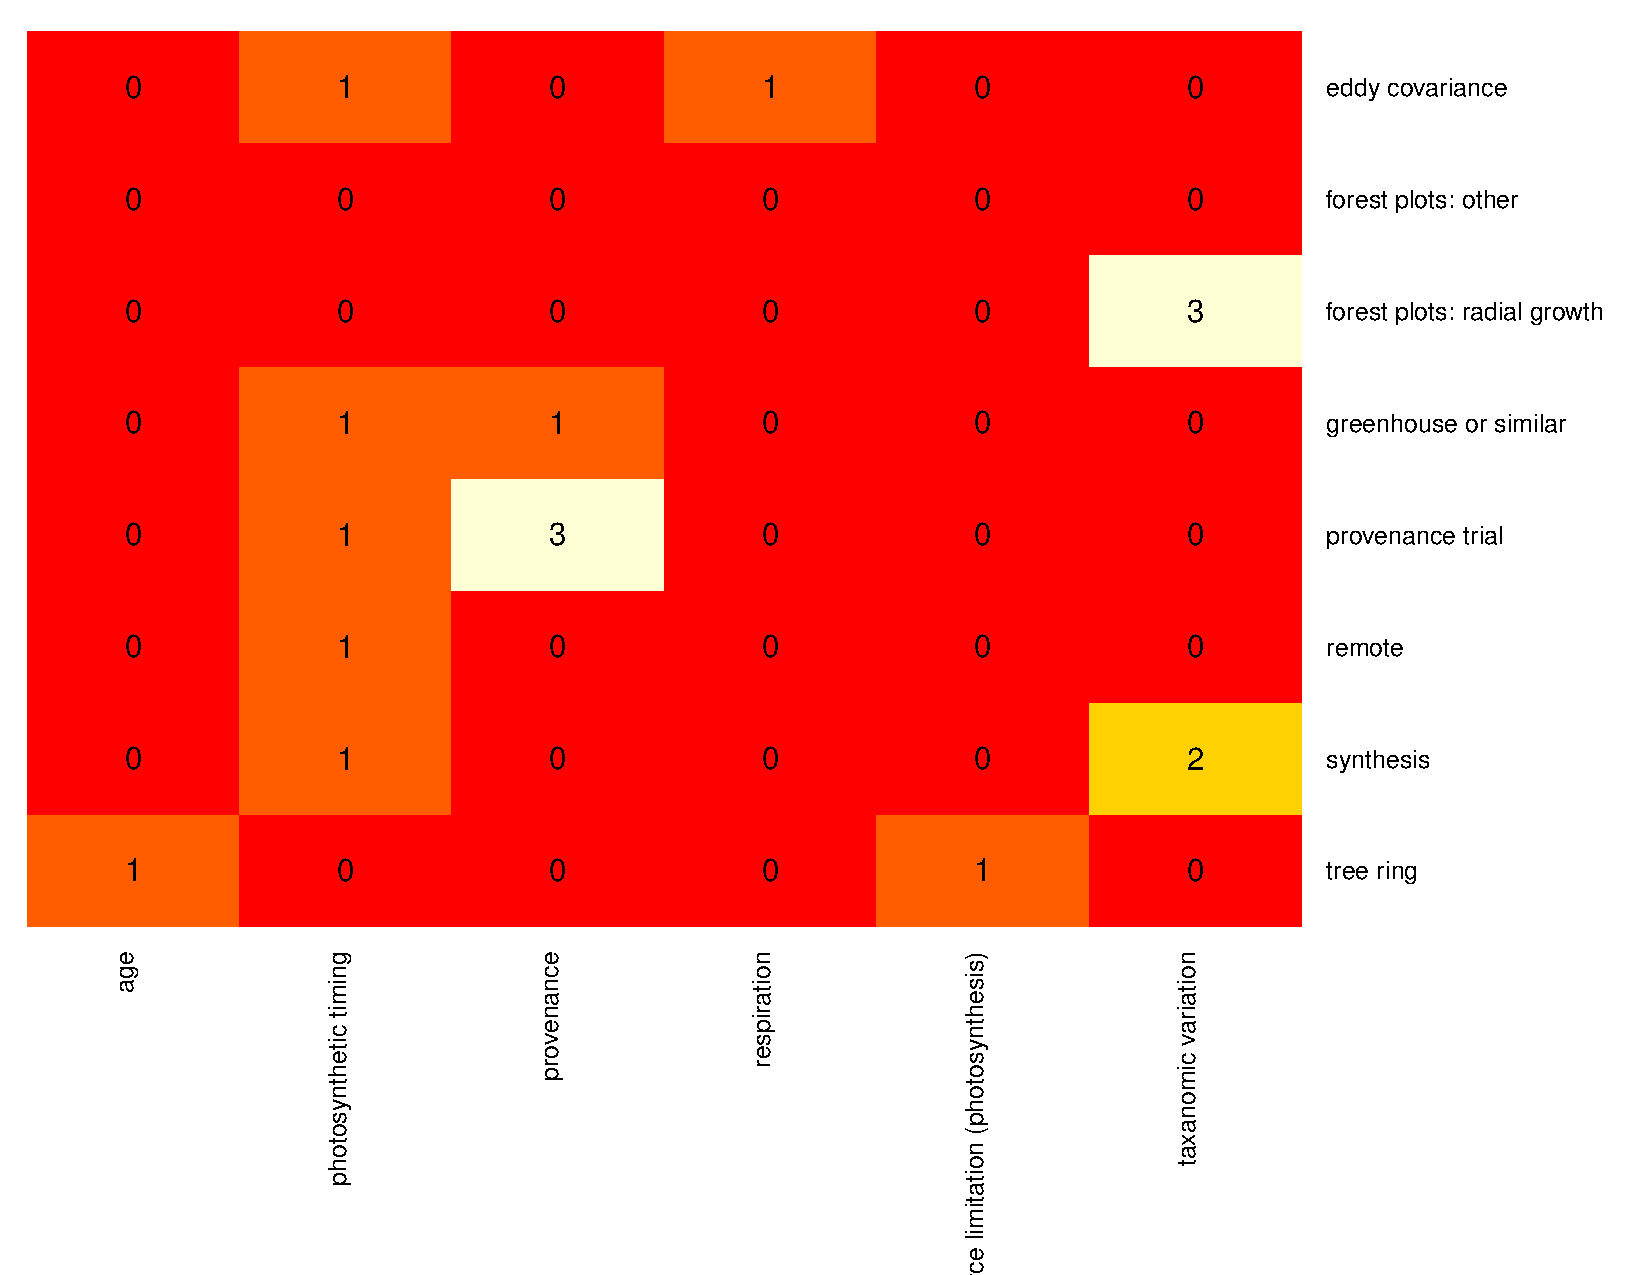
\includegraphics[width=0.8\textwidth]{..//figures/heatmaps/heatmap_endobymethod.pdf}
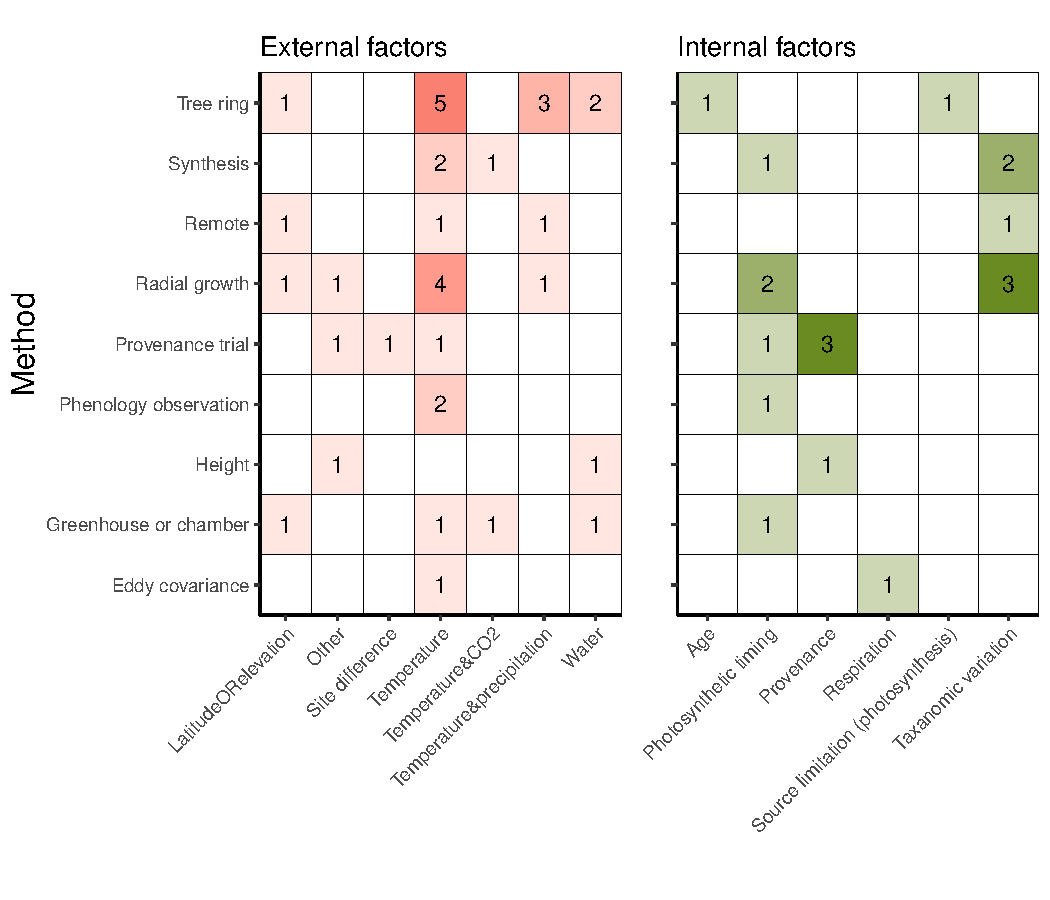
\includegraphics[width=0.8\textwidth]{..//figures/heatmaps/heatmap_combined_endo&exo.pdf}
\caption{A review of the prevalence of external (left) and internal (right) drivers mentioned in studies from our literature review, grouped by the general methods used. Many studies tested related hypotheses by measuring different drivers (e.g., latitude or elevation), so we combined similar external and internal factors for clearer comparisons.}
\label{fig:heatmapssupp}
\end{figure}

\clearpage
\begin{figure}[h!]
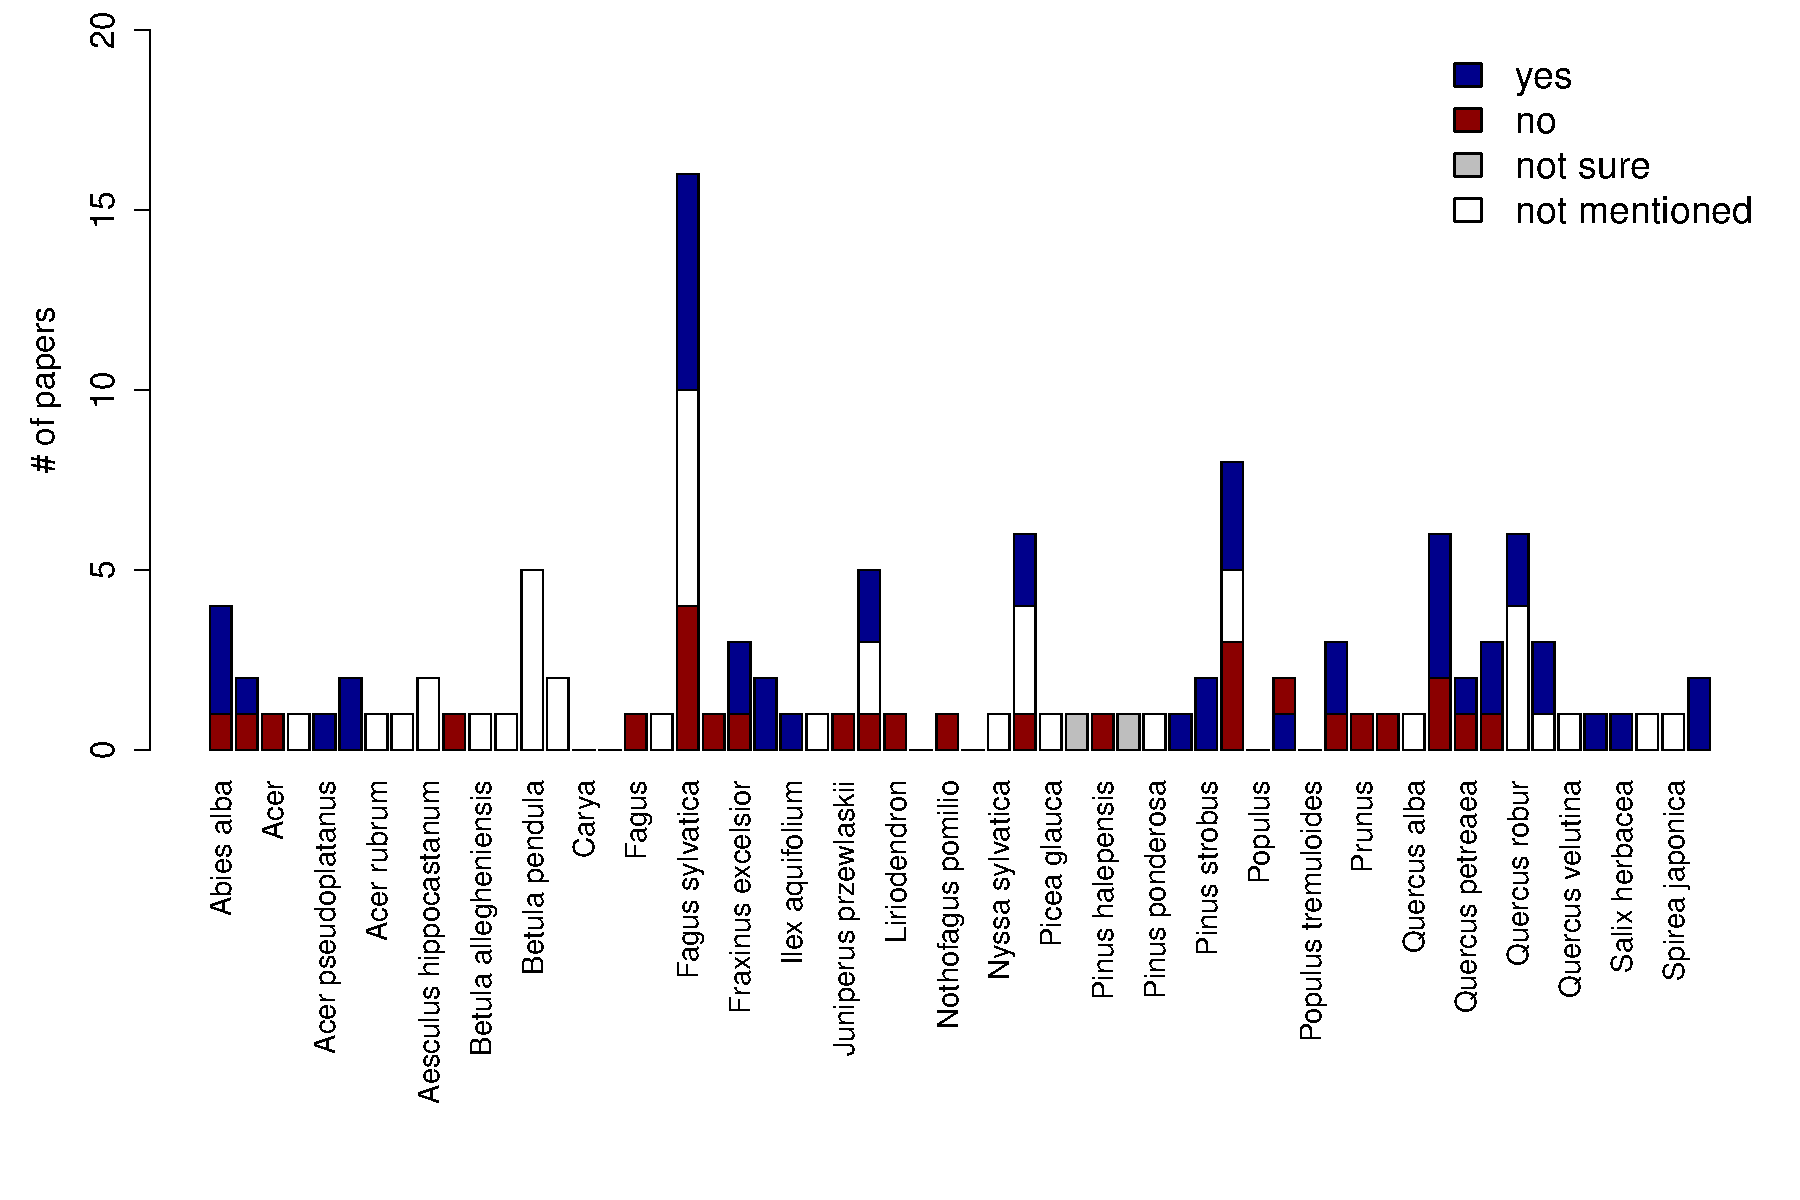
\includegraphics[width=1\textwidth]{..//figures/speciesnums_finds.pdf}
\caption{Results of whether studies found a relationship between growth and growing season length were generally inconsistent across  and within species. `Yes' indicates a study found a positive growth $\times$ growing season length relationship, while a `no' means they did not. A number of studies tested relationships possibly related to growth $\times$ growing season length (e.g., they tested how spring temperatures related to growth) but never directly tested growth $\times$ growing season length, which are indicated by `not tested.'}
\label{fig:sppfinds}
\end{figure}

\clearpage
\begin{figure}[h!]
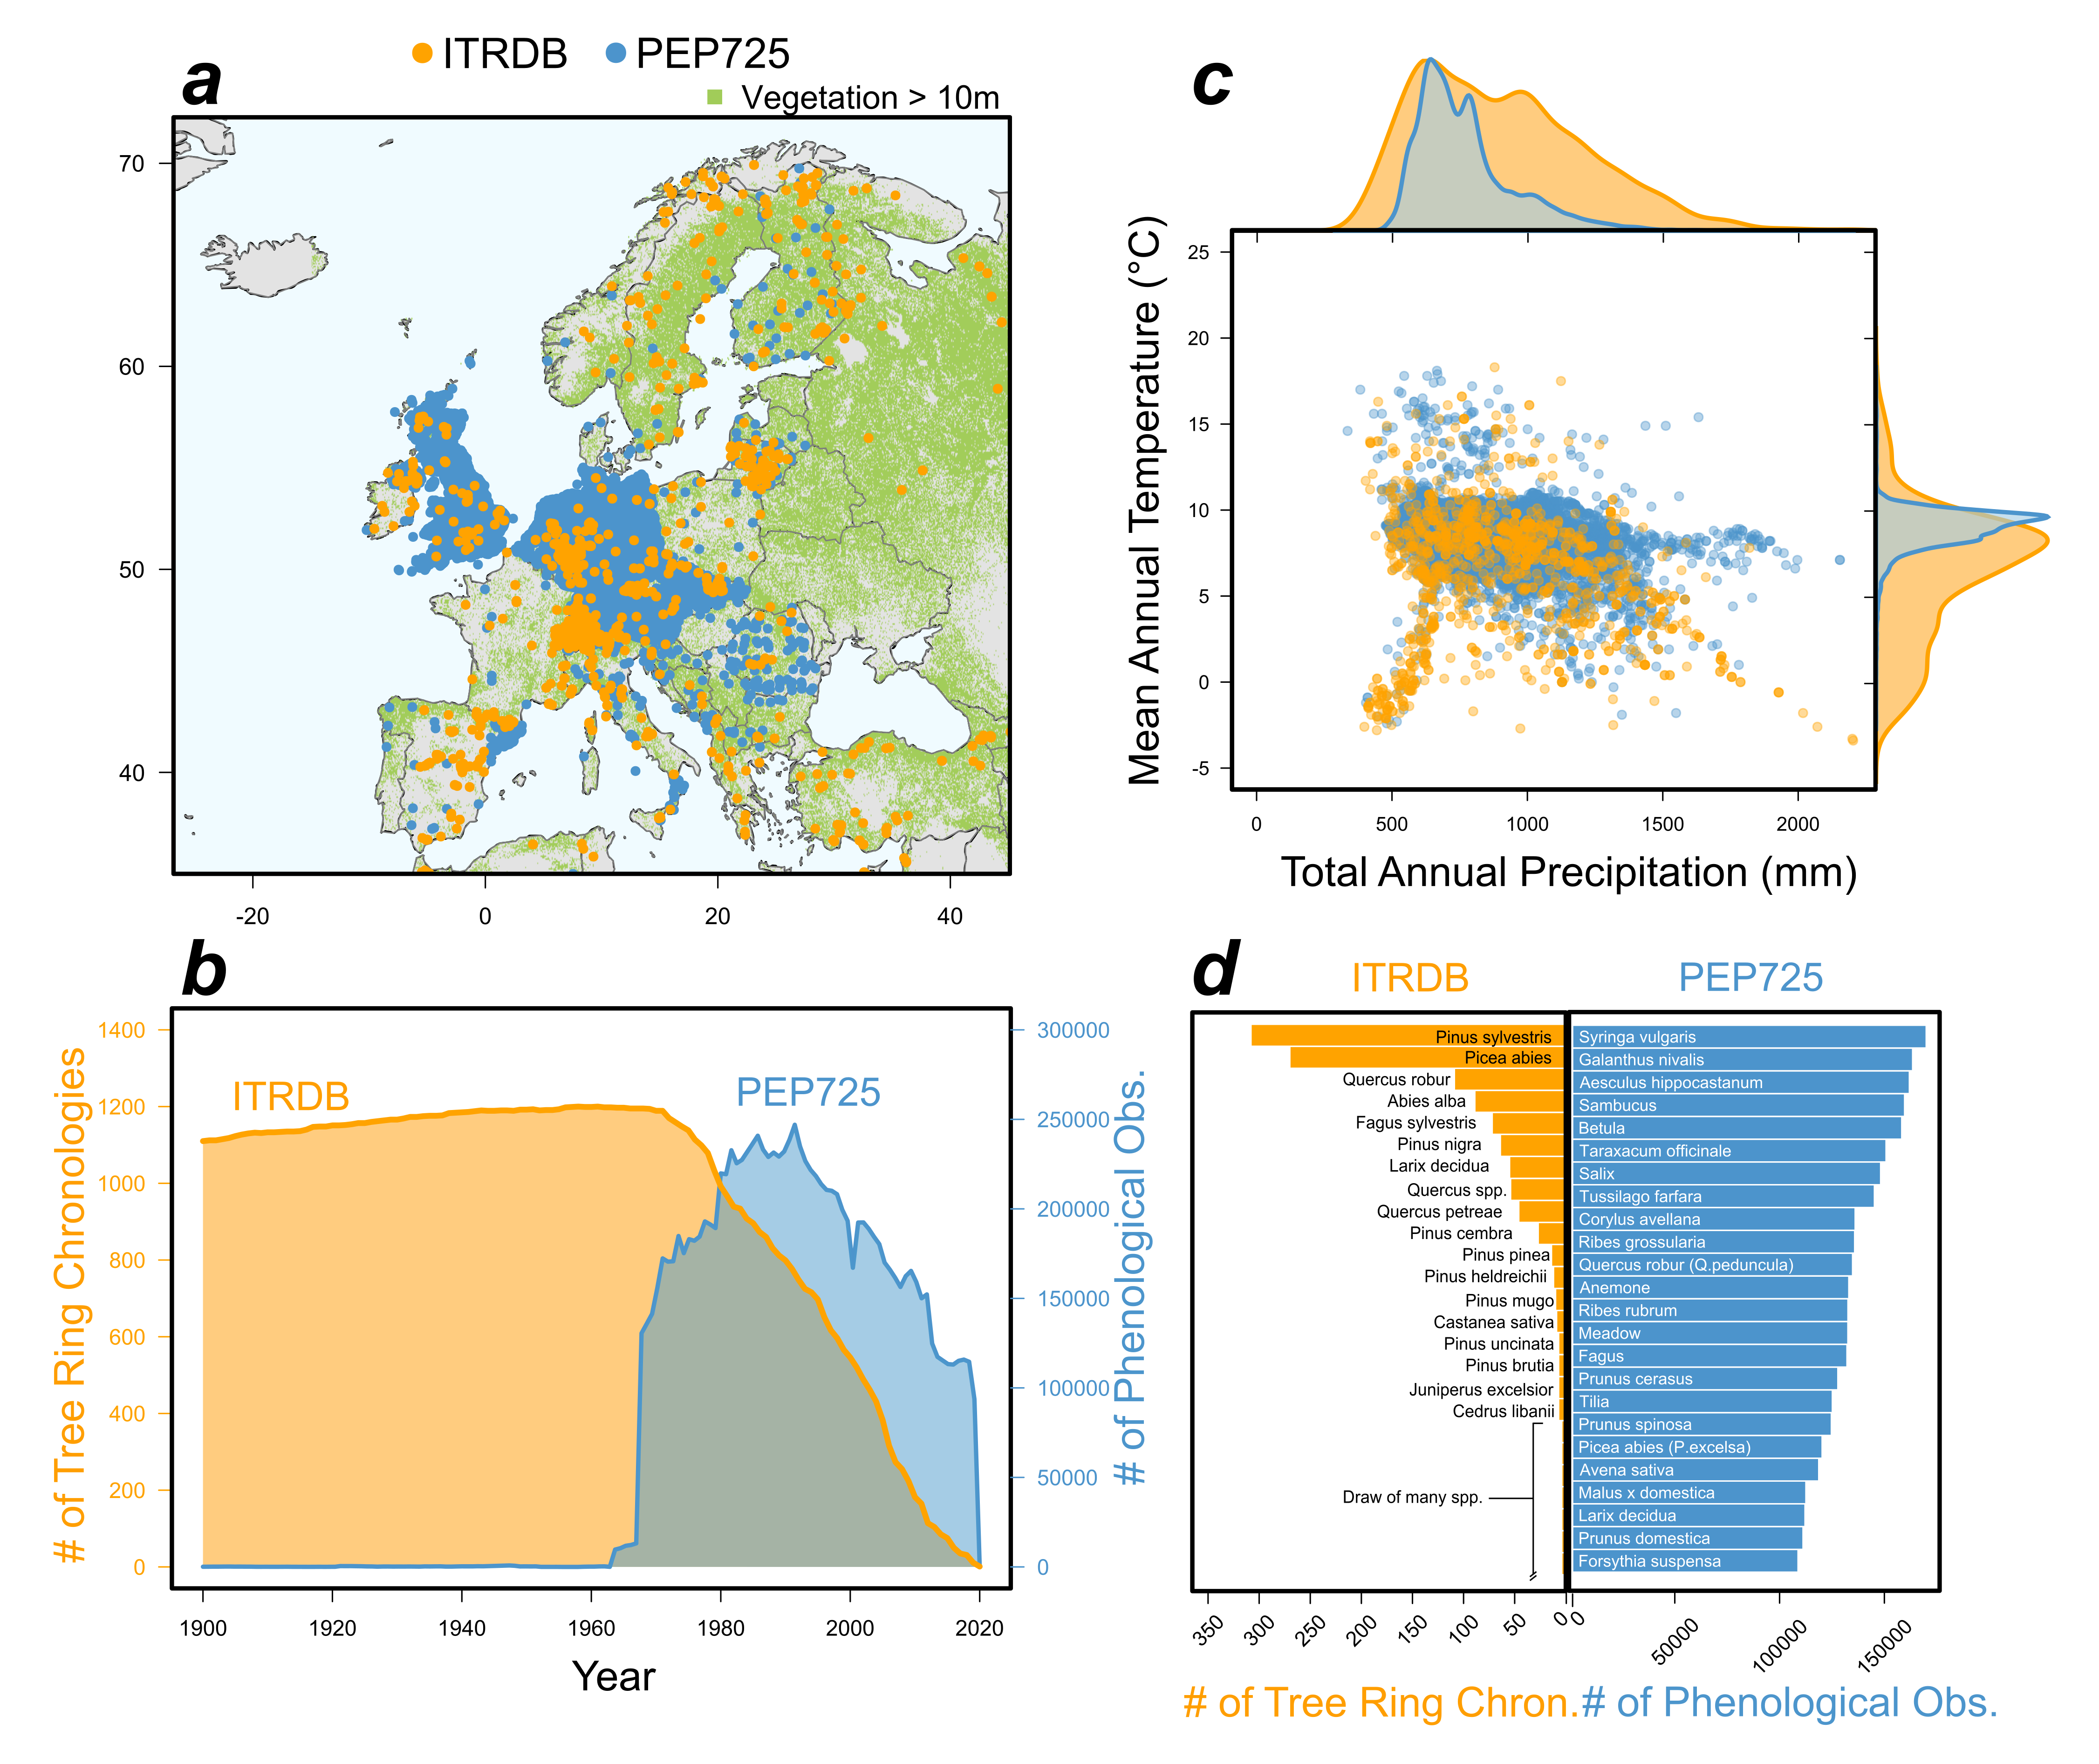
\includegraphics[width=1\textwidth]{..//figures/_figuresFromRuben/itrdb_vs_pep.png} %{..//figures/itrdbpep.png}
\caption{Data overlap between the two major databases of growth (International Tree Ring Data Bank, ITRDB, orange) and plant phenology (Pan European Phenology Project, PEP725, blue). Both databases are compared in terms of their spatial distributions (a), temporal overlaps (b), coverage of environmental conditions in climate space (c) and taxonomical representation (d). Note that the number of tree ring chronologies in (b) are composed by multiple trees per site, typically 10-20. Climatic data from Worldclim database ver. 2.1 at 2.5\degree grid resolution. PEP725 records in d) show the largest records for any given phenophase per species.}
\label{fig:itrbdpep}
\end{figure}


\clearpage
\section*{References}
\bibliography{..//bibtex/grephonbib}
\bibliographystyle{/Users/Lizzie/Documents/git/bibtex/styles/besjournals.bst}

\end{document}



\clearpage
\begin{figure}[h!]
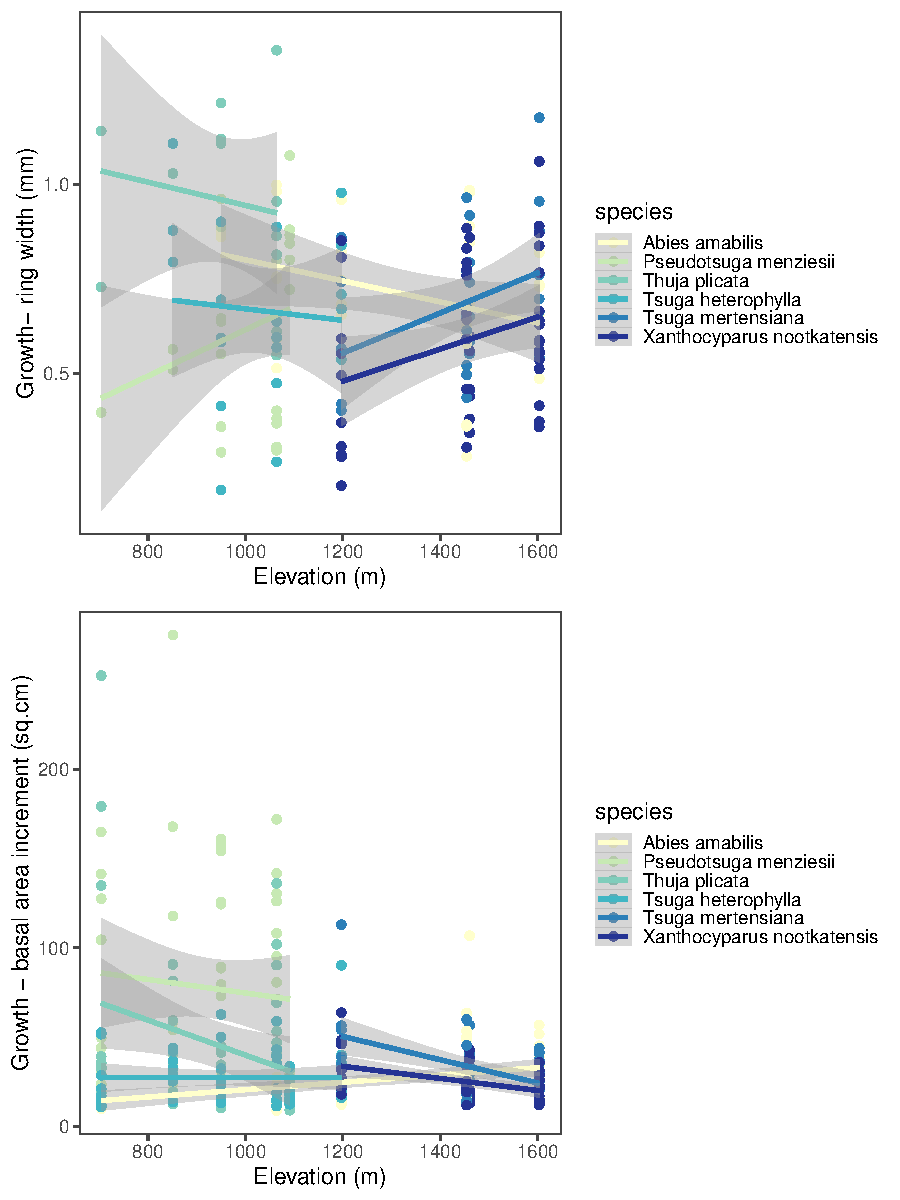
\includegraphics[width=0.7\textwidth]{..//analyses/growthxelevationetc/figures/grbyelev_rwvsbai_big}
\caption{Growth by elevation relationships for Mount Rainier (in development).}
\label{fig:growelevMORA}
\end{figure}

\section*{Towards standardized measurements \& tests}

 A common framework where researchers aim to report certain relevant drivers (e.g., several temperature and precipitation responses across the growing season) and broaden the metrics they use to encompass a standard set of growth and growing season length metrics....

While our lit review showed that the varying metrics of growth and growing season length can similarly find---or not find---a relationship, we also struggled to make scrape any consistent quantitative estimates---so metrics do matter intensely to helping the field progress. To start the conversation on a standardized set of measurements, we propose:
\begin{enumerate}
\item Ideal measure of growth
\begin{enumerate}
\item Annual increments seem best to me ... no? For long-term forest growth plots, ensuring annual growth measurements paired with phenological measurements would help (most permanent plot data I know of, e.g. FIA and PSP, is collected every 5 years, no phenology). 
\end{enumerate}
\item Ideal measures of wood and vegetative phenology: ideally at the individual level, as satellites cannot differentiate end of season well from herbivory and other factors. Also, given our focus on increment growth, wood phenology is best, but given how hard it is to collect these data we recommend wood phenology people also collect leaf phenology
\begin{enumerate}
\item Xylogenesis folks should measure ....
\item Vegetative: budburst and budset as gold standards for single stages, while photosynthetic measures critical for aligning with satellites etc.. Some of these are time intensive though, so---if you must report more qualitative measures, such as leaf coloring or leaf drop---aim to report several.  
\end{enumerate}
\end{enumerate}

We should also agree on a standardized set of analytical tools. E.g. tree ring analyses --- average away a lot of the interesting things. I<U+2019>m sure there are issues with phenological data, not sure what they are. ... and people should just report direct tests of the relationship so we don't end up with so many `did not measure' answers (Fig. \ref{fig:heatmaps}). And should we recommend tests for lag effects?


